\section{Pre-simulation sanity checks and planning tips}
\label{sec:sanity}

Sampling a molecular system that is complex enough to be ``interesting'' in modern science is likely to be extremely challenging.
Therefore, a small amount of effort spent planning a study can pay off many, many times over: in the worst case, weeks or months of simulation time followed by additional weeks or months of analysis can lead to insignificant conclusions in a poorly planned study.

If you read this guide through \emph{before} performing a simulation, you will have a much better sense of the criteria applicable to your data -- and which indeed \emph{should} be applied by knowledgeable reviewers of your work.
Thus we strongly advise understanding the concepts presented here as well as in related reviews \cite{Grossfield2009,JCGM:GUM2008}.

In a generic sense, the overall goal is to be able to draw statistically significant conclusions regarding a particular phenomenon or question of interest.
And ``good statistics'' follow from repeated observations of a phenomenon, which can only happen if the simulation length \emph{exceeds} the pertinent timescales.

One general strategy that will allow you to at least understand your data in a self-consistent way is to perform several repeats of the same simulation protocol: as described below, repeats can be used to assess variance in \emph{any} observable, within the time you have run your simulation.
When performing simulation repeats, it is sometimes suggested to use different starting states which are as diverse as possible; then, differences among the runs can be an indicator of inadequate sampling of the equilibrium distribution.
Alternatively, performing multiple runs from the same starting state will yield behavior particular to that starting state and potentially equilibrium if the runs are long enough.

What are the pertinent timescales?
That's a question which has to be answered individually for each system.
You will want to study the experimental and computational literature for your particular system, although we warn that a published prior simulation of a given length does not in itself validate a new simulation of a similar or slightly increased length.
In the end, your data must be validated as well as possible by statistical analyses, such as those described below. 
Be warned that a system may possess states (regions of configuration space) that, although important, are \emph{never} visited in a given simulation set because of insufficient computational time \cite{Grossfield2009} -- and this type of error will not be discovered through the analyses presented below.
Finally, note that "system" here does not necessarily refer to a complete biological simulation (e.g. protein, solvent, ions, etc) - it can also refer to some subset of the simulation for which data is desired. 
For example, if one is only interested in the dynamics of a binding site in a protein, it probably is not necessary to observe the unfolding and refolding of that protein as well.


\begin{figure}
  \centering
  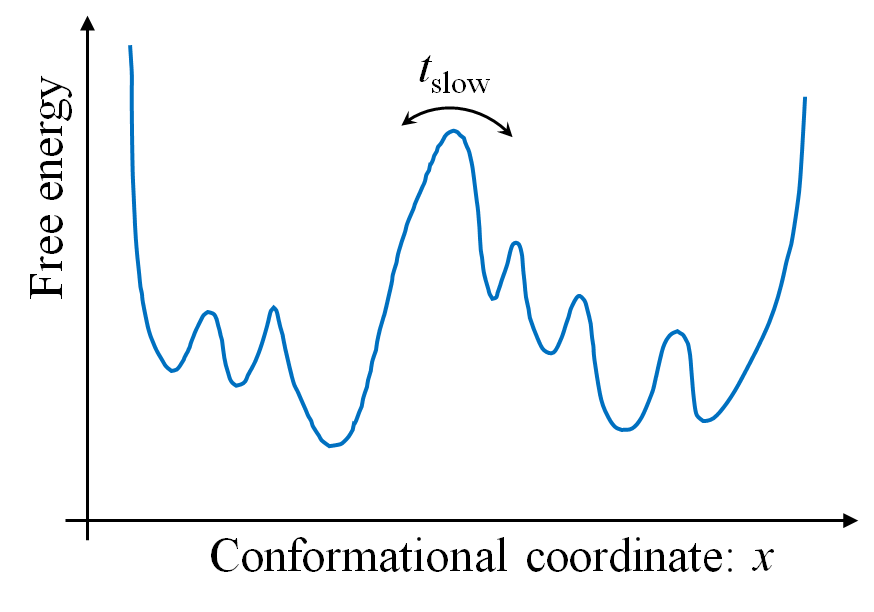
\includegraphics[width=5.8cm]{figures/1d-landscape-tslow}
  \caption{
  \label{fig:landscape} 
  Schematic illustration of a free energy landscape dominated by a slow process.
  The timescales associated with a system will often reflect ``activated'' (energy-climbing) processes, although they could also indicate diffusion times for traversing a rough landscape with many small barriers.
  In the figure, the largest barrier is associated with the slowest timescale $t_{\mathrm{slow}}$, and the danger for conventional MD simulations is that the total length of the simulation may be inadequate to generate the barrier crossing.
  The presence of stochasticity implies that even a simulation as long as $t_{\mathrm{slow}}$ may not yield the key event.
  }
\end{figure}

A toy model can generically illustrate timescales and their effects on sampling.
Consider the double-well free energy landscape shown in Fig.\ \ref{fig:landscape}, noting the slowest timescale is for crossing the largest barrier.
Generally, you should expect that the value of \emph{any} observable (e.g., $x$ itself or another coordinate not shown or a function of those coordinates) will depend on which of the two dominant basins the system occupies; and, in turn, the equilibrium average of an observable will require sampling the two basins according to their equilibrium populations.
In order to directly sample the equilibrium populations of the two basins, the length of a trajectory will have to be many times the slowest timescale, i.e. the largest barrier should be crossed multiple times.
The relative populations of states are inferred from time spent in each state, which only will be representative if there are many transitions;
put another way, the equilibrium populations follow from the transition rates \cite{Zuckerman2011} which can be estimated from multiple events.
For completeness, we note that there is no guarantee that sampling of a given system will be limited by a dominant barrier.  
Instead, a system could exhibit a generally rough landscape with many pathways between states of interest.
Nevertheless, the same cautions apply.

What should be done if a determination is made that a system's timescales are too long for direct simulation?
The two main options would be to consider a more simplified (``coarse-grained'') model or an enhanced sampling technique, bearing in mind that enhanced sampling methods are not foolproof but have their own limitations which should be considered carefully.

Lastly, whatever simulation protocol you pursue, be sure to use a well-validated piece of software [\url{https://github.com/shirtsgroup/software-physical-validation}].
If you are using your own code, check it against independent simulations on other software for a system that can be readily sampled.
%[benchmark systems???]

